\chapter{Architectural Views} \label{ArchitecturalViews}

\section{Context View}

\subsection{Stakeholders’ uses of this view}
The Context View is utilized by various stakeholders to understand how FarmBot interfaces with its environment and other systems:
\begin{itemize}
    \item \textbf{Hobbyist Gardeners and Professional Farmers:} They might consult the Context View to grasp how FarmBot integrates with weather services, plant databases, and other agricultural tools, enhancing their ability to use FarmBot effectively within their existing workflows.
    \item \textbf{Educators:} Educators leverage the Context View to illustrate to students the broader ecosystem of FarmBot, including its connectivity to cloud services and the exchange of information between FarmBot and external agricultural knowledge bases.
    \item \textbf{Researchers:} Researchers examine the Context View to ascertain how their experimental designs will interact with the various components of FarmBot, and to ensure the integrity of data exchange for their studies.
    \item \textbf{Software Developers:}  Developers rely on the Context View to conceptualize how the different pieces of the FarmBot software interact with the hardware components, the Web Application, and third-party APIs like OpenFarm.cc.
    \item \textbf{System Administrators:} Admins use the Context View to monitor and maintain the health of the system, ensuring the integration points between FarmBot and external services are functioning as expected.
    \item \textbf{Open-Source Contributors and Community Members:} They might use the Context View to better understand where their contributions can be most effective and how to interface with FarmBot's various system components.
\end{itemize}
Each stakeholder interacts with the Context View based on their unique concerns and needs, ensuring they can effectively engage with and support the FarmBot system.

\subsection{Context Diagram}
\begin{figure}[htbp]
    \centering
    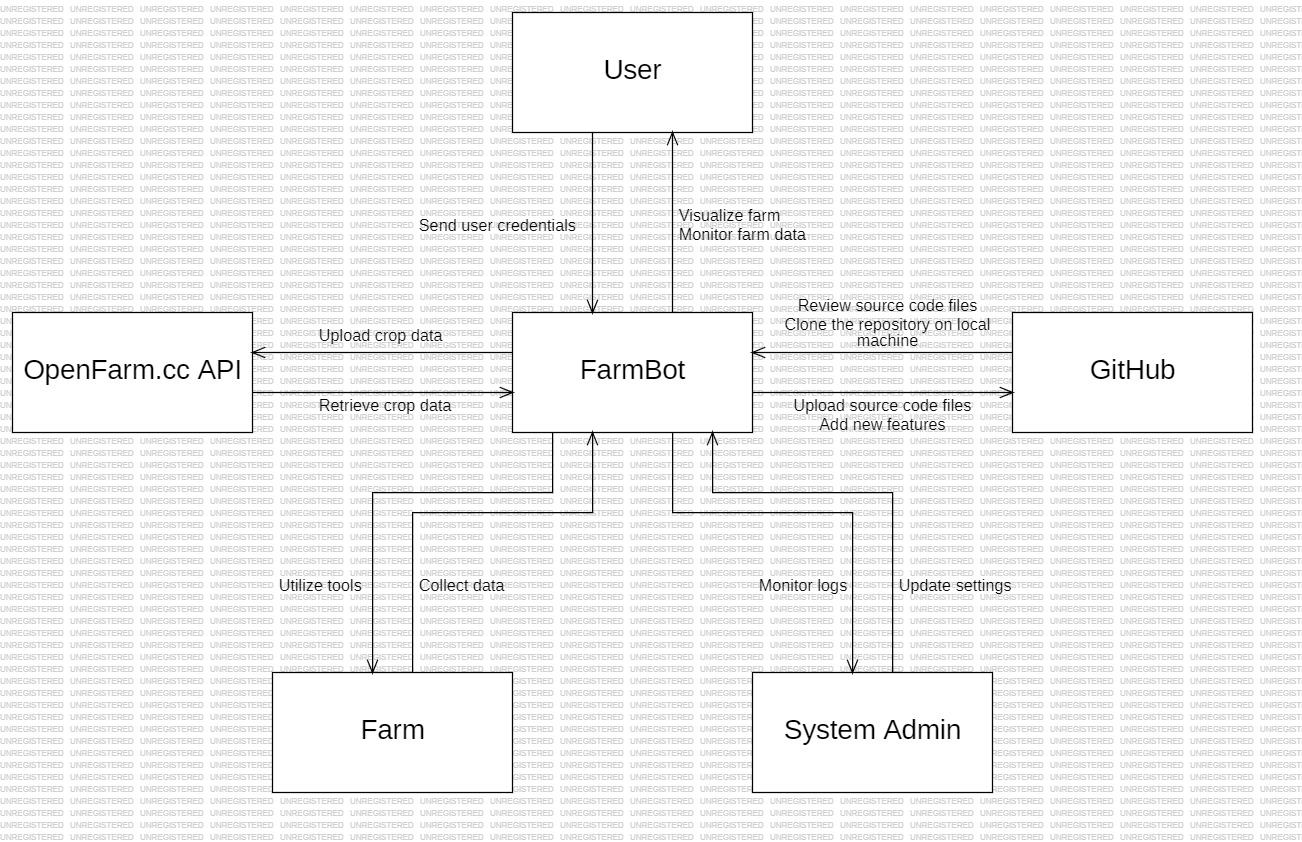
\includegraphics[width=1\linewidth]{Figures/context_diagram.jpg}
    \caption{System Context Diagram}
    \label{ContextDiagram}
\end{figure}
\newpage
The FarmBot system operates as an independent entity, interfacing with various external components to enhance its autonomous agricultural capabilities. Key interactions include:
\begin{itemize}
    \item \textbf{OpenFarm.cc API:} FarmBot utilizes this service to enrich its database with extensive plant cultivation data, enabling users to make informed decisions about crop management and optimizing agricultural practices.
    \item \textbf{User:} Individuals engage directly with FarmBot, providing their credentials to gain personalized access, and in return, they receive visual and data-driven insights into the farm's operations, contributing to an interactive farming experience.
    \item \textbf{System Admin:} This role is critical to the health of the FarmBot system, involving the monitoring of logs, the collection of data, and the adjustment of settings to ensure optimal performance.
    \item \textbf{GitHub:} Serves as a collaborative platform for the FarmBot community, where developers and contributors manage the codebase, addressing system enhancements, bug fixes, and feature requests.
    \item \textbf{Farm:} The physical environment where FarmBot's tools are deployed, and data is collected to perform a variety of tasks such as planting, watering, and monitoring environmental conditions.
\end{itemize}
The context diagram emphasizes the balance between user interaction, automated farming processes, and data exchange, ensuring that FarmBot functions as a cohesive system for sustainable and technologically advanced agriculture.

\newpage
\subsection{External Interfaces}
\begin{figure}[htbp]
    \centering
    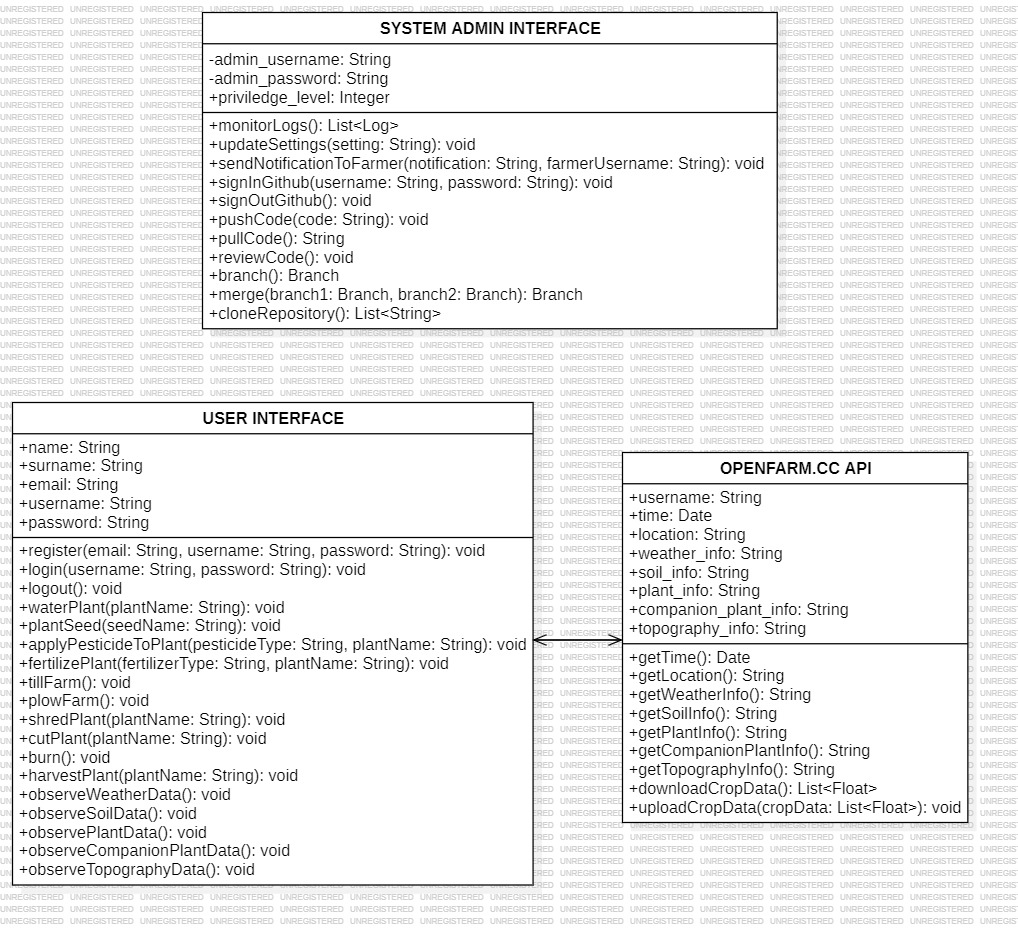
\includegraphics[width=1\linewidth]{Figures/external_interfaces.jpg}
    \caption{External Interfaces Class Diagram}
    \label{ExternalInterfaces}
\end{figure}
\newpage
In the architecture of the FarmBot system, external interfaces play a pivotal role in seamless interaction between users, administrators, and the broader online community. Here is an overview of each interface's core functionalities:
\begin{itemize}
    \item \textbf{User Interface:} Acts as the direct touchpoint for users to manage and interact with FarmBot's diverse agricultural tasks such as planting and harvesting, leveraging a straightforward design that accommodates varying levels of user expertise. Methods and fields of this interface
    can be described as follows:
    \begin{itemize}
        \item \textbf{name, surname, email:} Personal identification fields for user accounts.
        \item \textbf{username, password:} Credentials for the user.
        \item \textbf{register}$()$, \textbf{login}$()$, \textbf{logout}$()$: Operations for signing in and signing out from the FarmBot application.
        \item \textbf{waterPlant}$()$: Command to initiate the watering of plants.
        \item \textbf{plantSeed}$()$: Function to start the planting of seeds.
        \item \textbf{applyPesticideToPlant}$()$: Function to apply pesticides to plants.
        \item \textbf{fertilizePlant}$()$: Command to fertilize plants.
        \item \textbf{tillFarm}$()$: Operation for tilling the soil.
        \item \textbf{plowFarm}$()$: Function to plow the farm area.
        \item \textbf{shredPlant}$()$: Command to shred unwanted plants.
        \item \textbf{cutPlant}$()$: Function to cut or prune plants.
        \item \textbf{burn}$()$: Command that could relate to a controlled burn function for crop management.
        \item \textbf{harvestPlant}$()$: Function to initiate the harvesting of plants.
        \item \textbf{observeWeatherData}$()$: Function to display current and forecasted weather data.
        \item \textbf{observeSoilData}$()$: Function to display real-time soil data such as moisture levels, pH, and nutrient profiles.
        \item \textbf{observePlantData}$()$: Function to display detailed information about the plants.
        \item \textbf{observeCompanionPlantData}$()$: Function to display information about companion planting strategies.
        \item \textbf{observeTopographyData}$()$: Function to display information about topography data such as latitude, longitute, and altitude.
    \end{itemize}
    \item \textbf{System Admin Interface:} Tailored for administrators to perform system-level operations, including monitoring and updating settings, thus ensuring the robustness and reliability of FarmBot's service. Methods and fields of this interface are:
    \begin{itemize}
        \item \textbf{admin\_username, admin\_password:} Credentials for the system administrator.
        \item \textbf{priviledge\_level:} Determines the level of access and control the admin has.
        \item \textbf{monitorLogs}$()$: Function for monitoring system logs.
        \item \textbf{updateSettings}$()$: Command to update system settings.
        \item \textbf{sendNotificationToFarmer}$()$: Function to send notifications to farmers.
        \item \textbf{signInGithub}$()$, \textbf{signOutGithub}$()$: Operations for signing in to and signing out from the GitHub repository.
        \item \textbf{pushCode}$()$, \textbf{pullCode}$()$: Functions for pushing and pulling code, respectively, to and from the repository.
        \item \textbf{reviewCode}$()$: Command to review code changes.
        \item \textbf{branch}$()$, \textbf{merge}$()$: Operations for branching and merging code for version controlling purposes.
        \item \textbf{cloneRepository}$()$: Function to clone the repository for local work or backup.
    \end{itemize}
    \item \textbf{OpenFarm.cc API:} Serves as a conduit for accessing and uploading detailed plant cultivation data, which is crucial for informed farming decisions and enhancing FarmBot's agricultural database. Methods and fields of this interface can be listed as:
    \begin{itemize}
        \item \textbf{username, time, location:} Identifiers for the user and timing/location for the data retrieval or action.
        \item \textbf{weather\_info, soil\_info, plant\_info, companion\_plant\_info, topography\_info:} Data fields containing environmental and cultivation details.
        \item \textbf{getTime}$()$, \textbf{getLocation}$()$, \textbf{getWeatherInfo}$()$, \textbf{getSoilInfo}$()$, \textbf{getPlantInfo}$()$, \textbf{getCompanionInfo}$()$, \textbf{getTopographyInfo}$()$: Functions to retrieve the current time, location details, and environmental conditions as well as specific plant and soil information.
        \item \textbf{downloadCropData}$()$: Function to download data about crops.
        \item \textbf{uploadCropData}$()$: Function to upload new crop data to OpenFarm.CC.
    \end{itemize}
\end{itemize}

\newpage
\subsection{Interaction scenarios}
\begin{figure}[htbp]
    \centering
    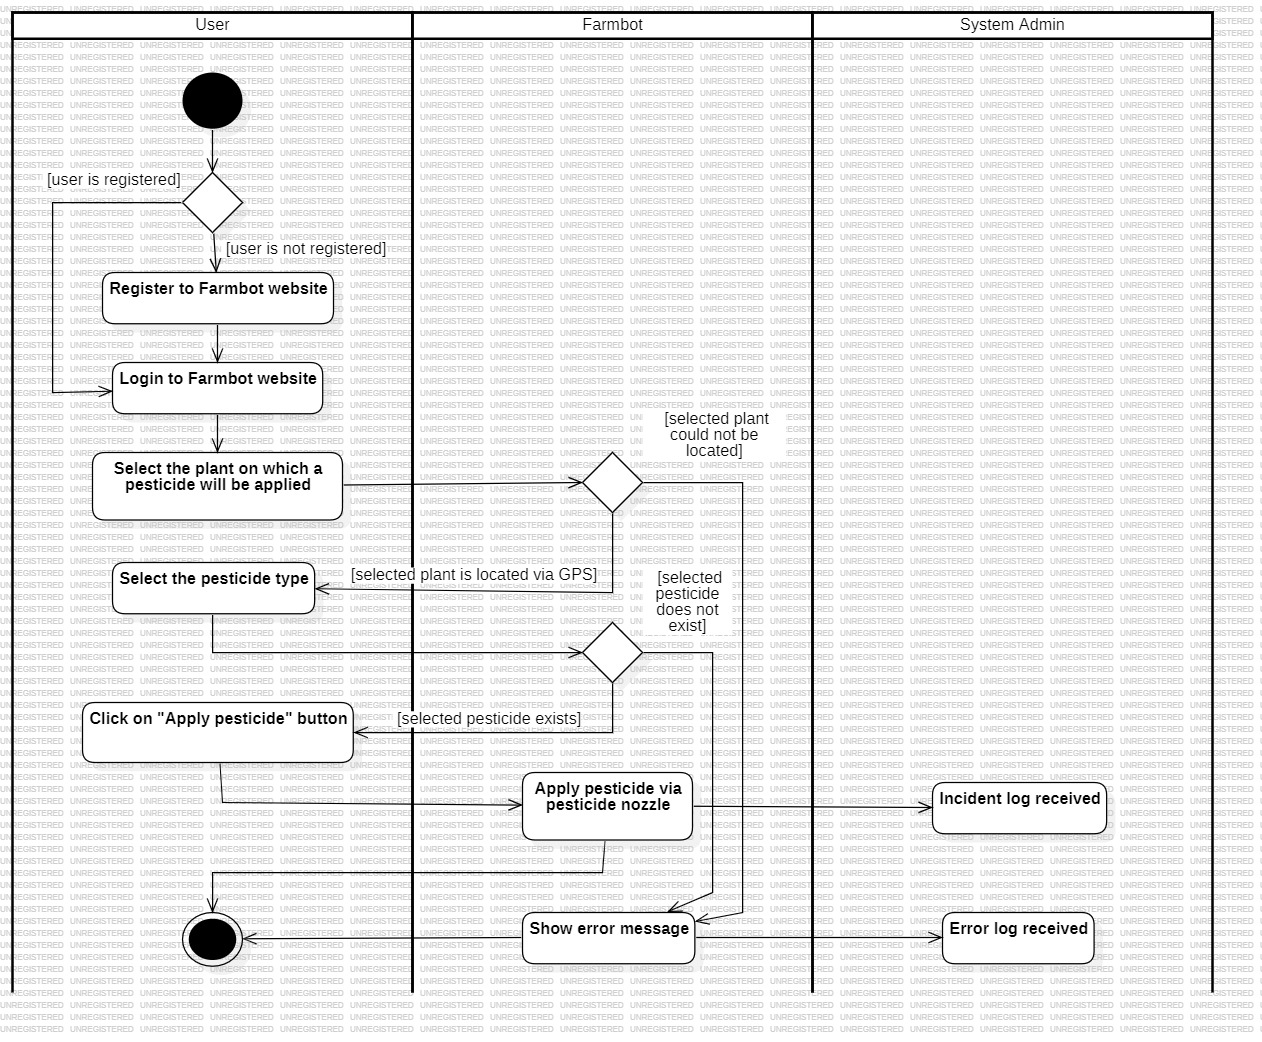
\includegraphics[width=1\linewidth]{Figures/activity1.jpg}
    \caption{Activity Diagram of the "Apply Pesticide to Plant" Interaction Scenario}
    \label{Activity1}
\end{figure}
\begin{figure}[htbp]
    \centering
    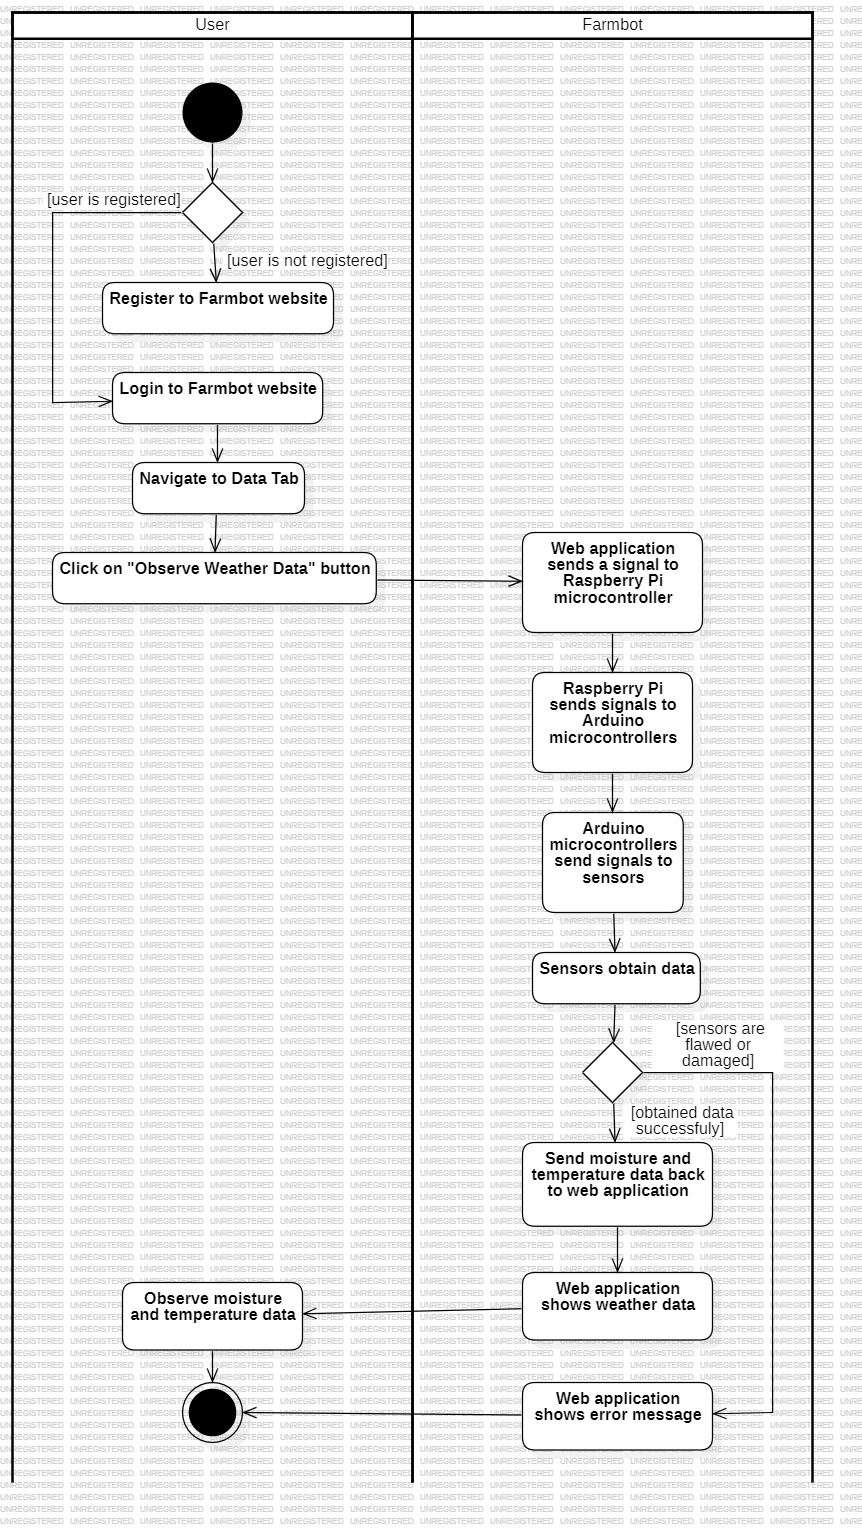
\includegraphics[scale=0.37]{Figures/activity2.jpg}
    \caption{Activity Diagram of the "Observe Weather Data" Interaction Scenario}
    \label{Activity2}
\end{figure}
\newpage

\section{Functional View}

\subsection{Stakeholders’ uses of this view}
The Functional View provides critical insights into the system's operations and interactions, with a primary focus on the diverse functionalities offered by FarmBot. The stakeholders of the FarmBot project, ranging from developers and users to administrators and contributors, utilize this view for various purposes:
\begin{itemize}
    \item \textbf{Developers:} Leverage the Functional View as a blueprint for understanding system operations, guiding them in creating functionalities. It also aids in identifying inter-component dependencies, essential for efficient code integration and system testing.
    \item \textbf{Users (Hobbyist Gardeners, Professional Farmers, and Educators):} Access the Functional View to comprehend the capabilities of FarmBot and how they can employ these features for automated farming, educational purposes, or agricultural research.
    \item \textbf{System Admins:} Utilize this view to monitor the efficacy of FarmBot's functions and to anticipate the impact of system updates or configurations.
    \item \textbf{Researchers:} Rely on the Functional View to investigate how FarmBot's features can be employed for experimental setups, data collection, and analysis, supporting their work in sustainable agriculture.
    \item \textbf{Contributors (Open-Source Community Users):} Use this view to see how their contributions fit into the broader FarmBot ecosystem and influence its functionality.
\end{itemize}
This Functional View acts as a lens through which the entire FarmBot operation can be understood, providing clarity to stakeholders about how their individual interactions with the system contribute to its goals of efficiency, sustainability, and user accessibility.

\subsection{Component Diagram}
\begin{figure}[htbp]
    \centering
    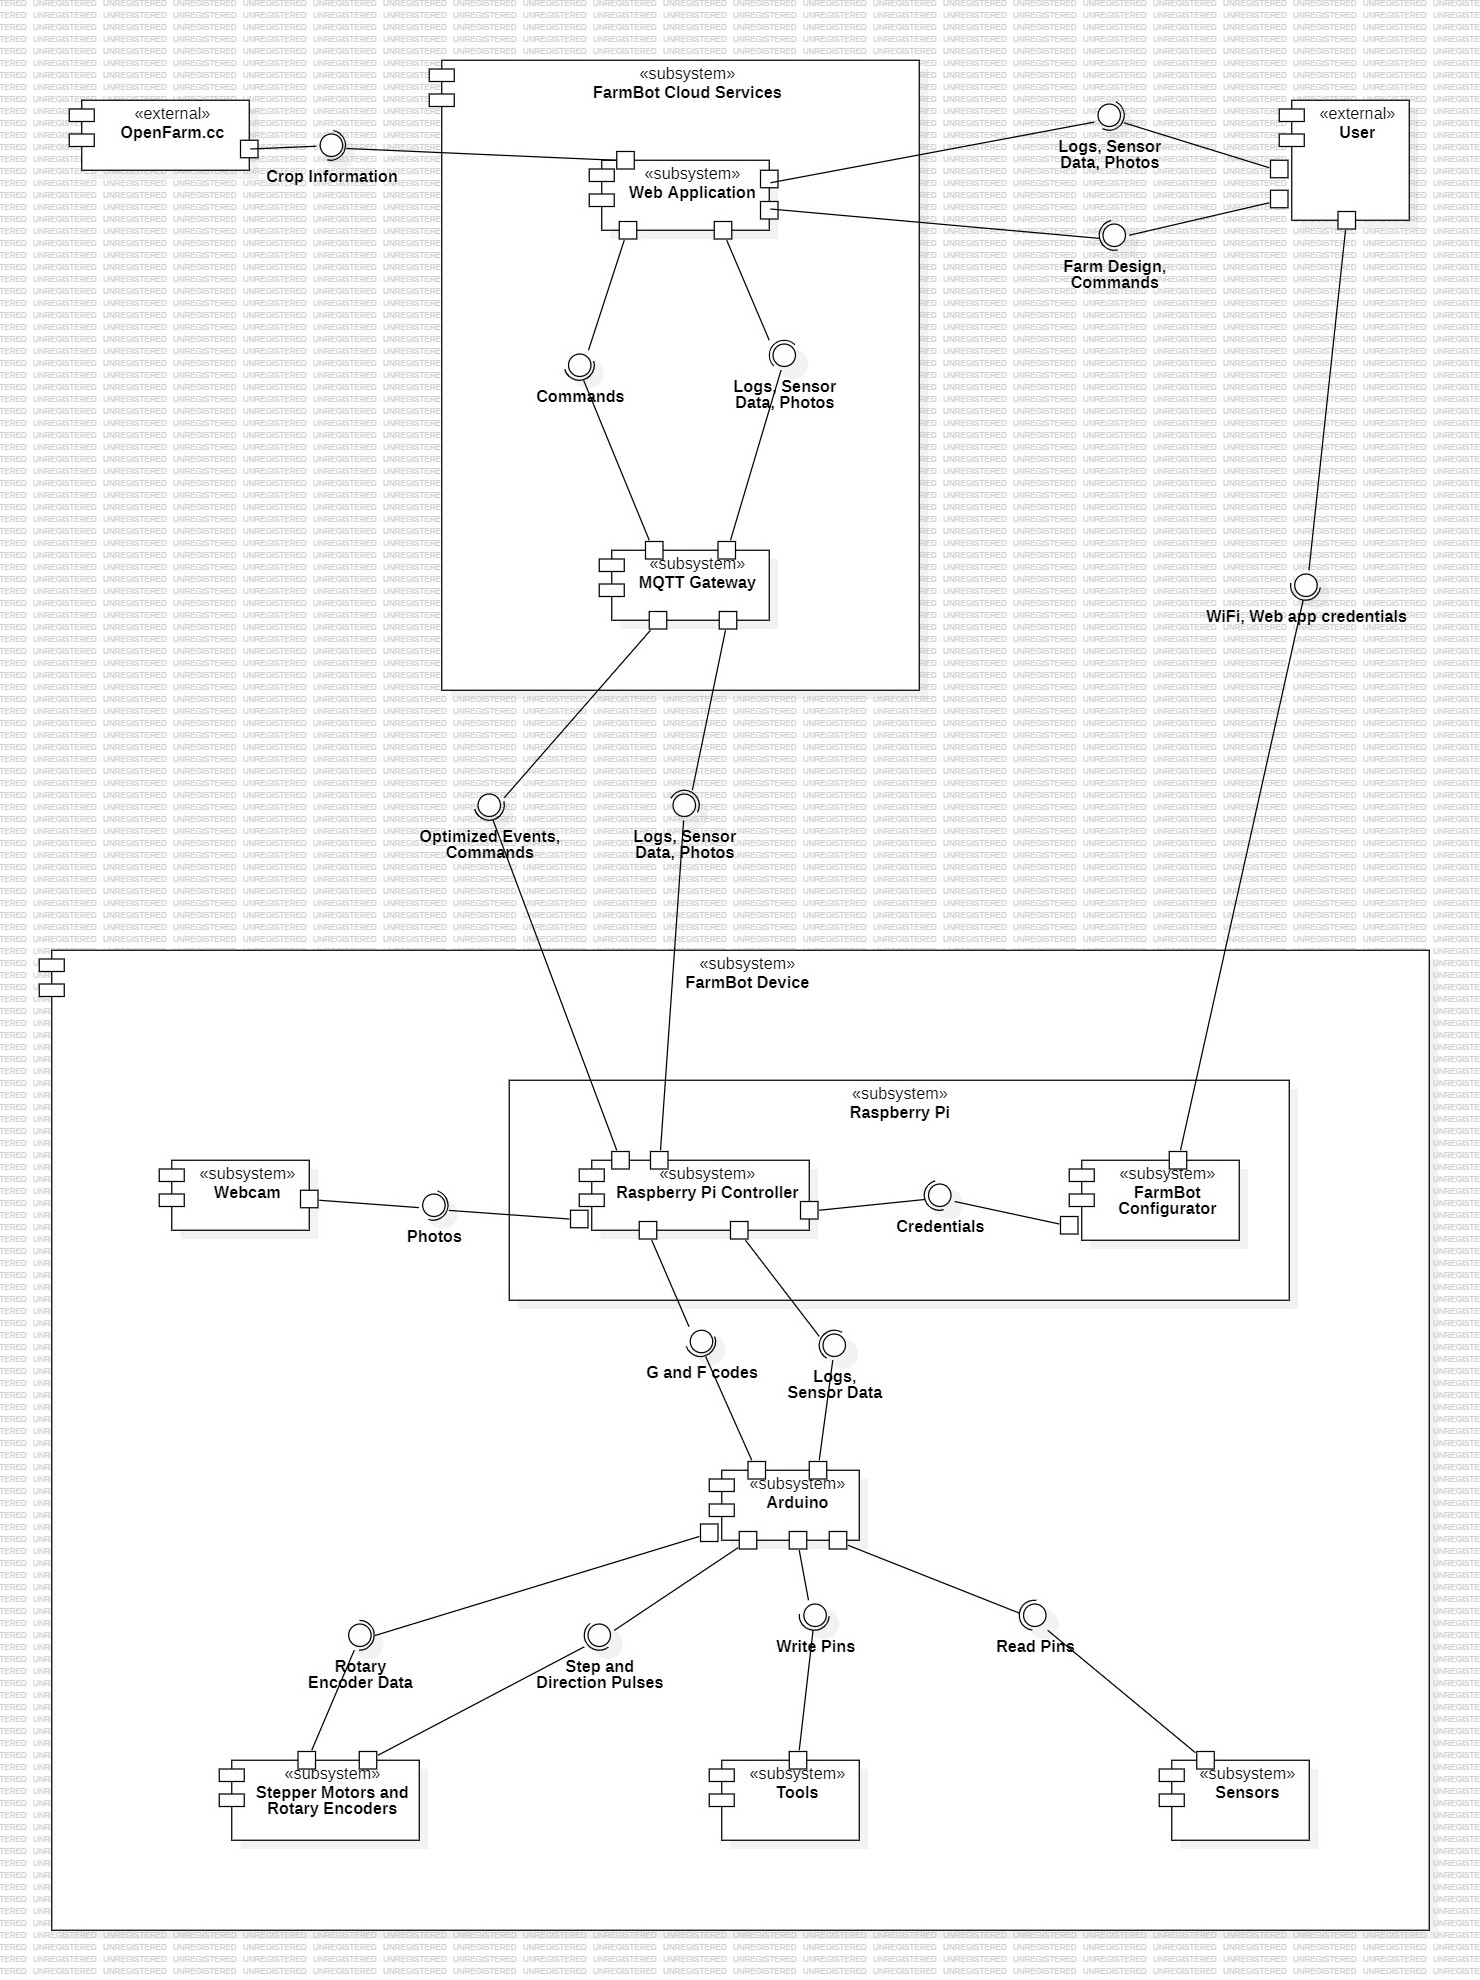
\includegraphics[width=0.7\textwidth]{Figures/component_diagram.jpg}
    \caption{Component Diagram}
    \label{Component}
\end{figure}
\newpage
The FarmBot system is composed of several interconnected subsystems: FarmBot Cloud Service, Web Application, MQTT Gateway, FarmBot device, Raspberry Pi, Webcam, FarmBot Configurator, Arduino, Stepper Motors \& Rotary Encoders, Tools and Sensors. These subsystems are structured into hierarchies for efficient management and operation. For instance, the FarmBot Cloud Service encompasses the Web Application and MQTT Gateway, while the FarmBot Device integrates components like the Raspberry Pi, Webcam, FarmBot Configurator, Arduino, Stepper Motors \& Rotary Encoders, and Tools and Sensors.\\\\
Within the FarmBot Cloud Service, the Web Application provides a user-friendly interface for configuring and managing the FarmBot operations. It facilitates the design of farm layouts, scheduling tasks, and viewing operational data. The MQTT Gateway acts as a communication broker that manages the messaging between the FarmBot device and the web application, ensuring timely and secure data transfer.\\\\
The FarmBot Device subsystem is central to the operation, containing several critical components:
\begin{itemize}
    \item \textbf{Raspberry Pi:} Acts as the control hub, processing commands from the web application and managing device operations.
    \item \textbf{Webcam:} Captures real-time visual data of the farm, which is accessible via the web application for monitoring and decision-making.
    \item \textbf{FarmBot Configurator:} A setup tool that helps users initialize the device by connecting it to their network and configuring its settings.
    \item \textbf{Arduino:} Interfaces directly with physical components, interpreting G-code instructions to operate the motors, tools, and read sensor data.
    \item \textbf{Stepper Motors \& Rotary Encoders:} These components drive the precise movement of the FarmBot along its tracks and provide feedback on position for accuracy.
    \item \textbf{Tools and Sensors:} Include various implements such as seed injectors, soil sensors, and watering nozzles that perform the actual agricultural tasks.
\end{itemize}
Each of these components works in harmony to ensure that the FarmBot operates efficiently, adhering to the precision farming model. The system's architecture supports scalability and modularity, allowing for future expansions and modifications to enhance capabilities or integrate new technologies as they become available. This structured yet flexible setup ensures that FarmBot can adapt to various farming environments and requirements, promoting innovation and improvement in automated farming technology.

\newpage
\subsection{Internal Interfaces}
\begin{figure}[htbp]
    \centering
    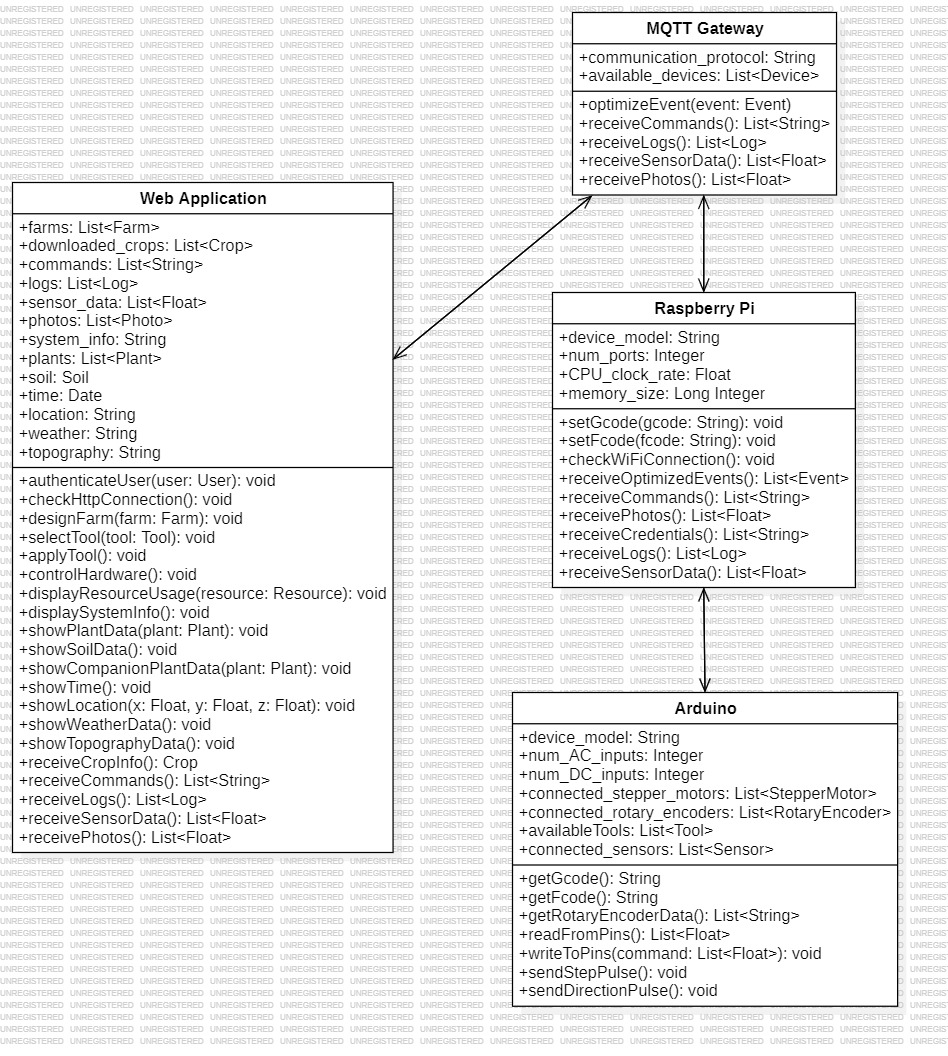
\includegraphics[width=0.9\linewidth]{Figures/internal_interfaces.jpg}
    \caption{Internal Interfaces Class Diagram}
    \label{InternalInterfaces}
\end{figure}
\newpage
FarmBot integrates a sophisticated combination of internal interfaces, each tasked with specific functions vital to the system’s operation. These interfaces enable seamless communication and operational coordination among the various components of FarmBot.
\begin{itemize}
    \item \textbf{Web Application Interface:} Acts as the primary user interaction platform, facilitating a variety of functionalities:
        \begin{itemize}
            \item User Authentication and Connection Checks: authenticateUser, checkHttpConnection
            \item Farm Design and Tool Management: designFarm, selectTool, applyTool
            \item Hardware Control and Monitoring: controlHardware, displayResourceUsage, displaySystemInfo
            \item Data Display and Environmental Monitoring: showPlantData, showSoilData, showCompanionData, showTime, showLocation, showWeatherData, showTopographyData
            \item Data Reception: receiveCropInfo, receiveCommands, receiveLogs, receiveSensorData, receivePhotos
        \end{itemize}
    \item \textbf{MQTT Gateway Interface:} Manages real-time communication, data reception, and event optimization:
        \begin{itemize}
            \item Event Management and Data Reception: optimizeEvent, receiveCommands, receiveLogs, receiveSensorData, receivePhotos
        \end{itemize}
    \item \textbf{Raspberry Pi Interface:} Serves as the central processing unit within the FarmBot device, handling command execution and data reception:
        \begin{itemize}
            \item Command Setting and WiFi Connection Check: setGcode, setFcode, checkWiFiConnection
            \item Optimized Event and Data Reception: receiveOptimizedEvents, receivePhotos, receiveCredentials, receiveLogs, receiveSensorData
        \end{itemize}
    \item \textbf{Arduino Interface:} Directly controls the physical operations of FarmBot, interfacing with the mechanical systems and sensors:
        \begin{itemize}
            \item Code Retrieval and Sensor Data Handling: getGcode, getFcode, getRotaryEncoderData
            \item Pin and Motor Control: readFromPins, writeToPins, sendStepPulse, sendDirectionPulse
        \end{itemize}
\end{itemize}
Each interface is meticulously designed to ensure that FarmBot operates efficiently, responding accurately to user inputs and effectively managing the automation of farming tasks. This structured interface design promotes clarity in component responsibilities, making the system both maintainable and scalable.

\newpage
\subsection{Interaction Patterns}
\begin{figure}[htbp]
    \centering
    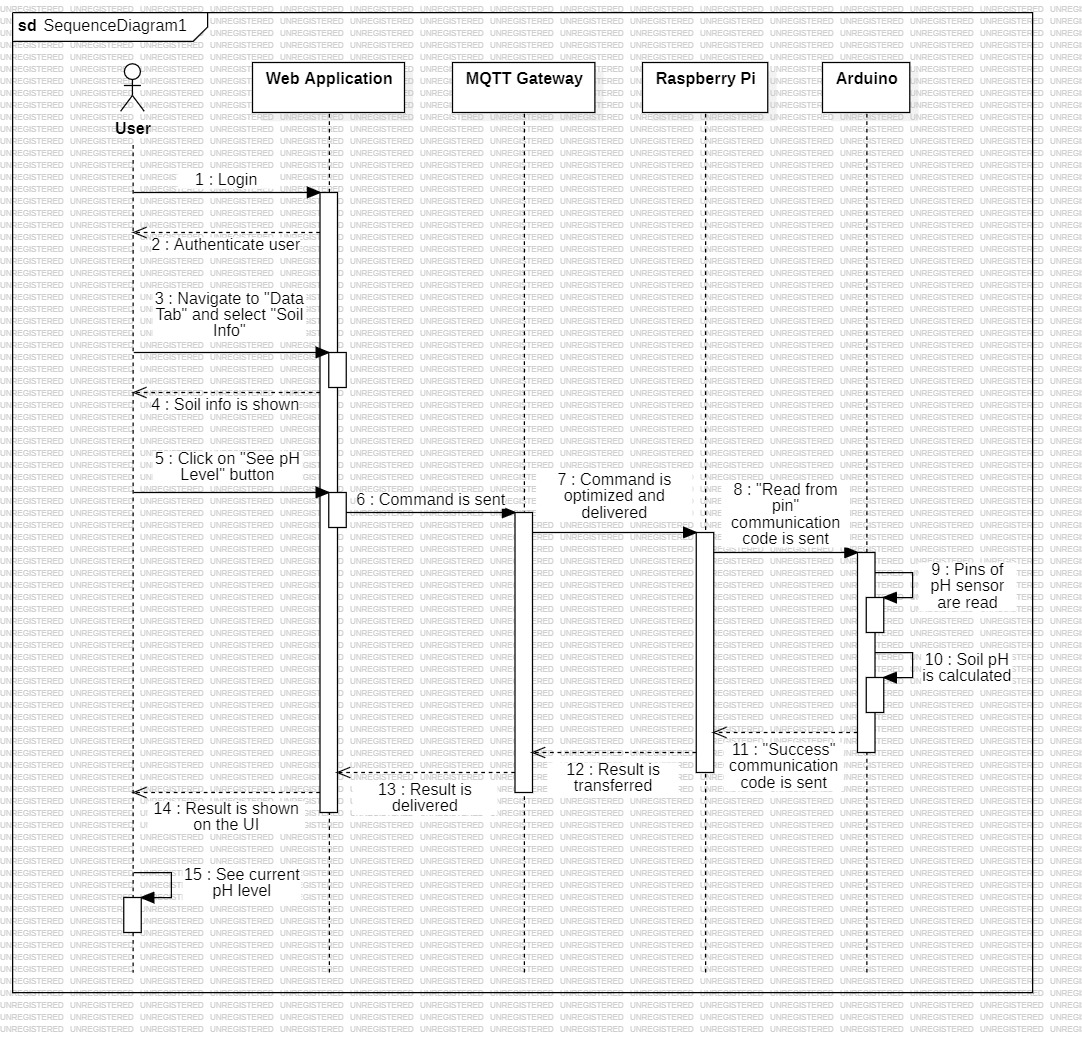
\includegraphics[width=1\linewidth]{Figures/sequence1.jpg}
    \caption{Sequence Diagram for "Show Current pH Level" Interaction Pattern}
    \label{Sequence1}
\end{figure}
\begin{figure}[htbp]
    \centering
    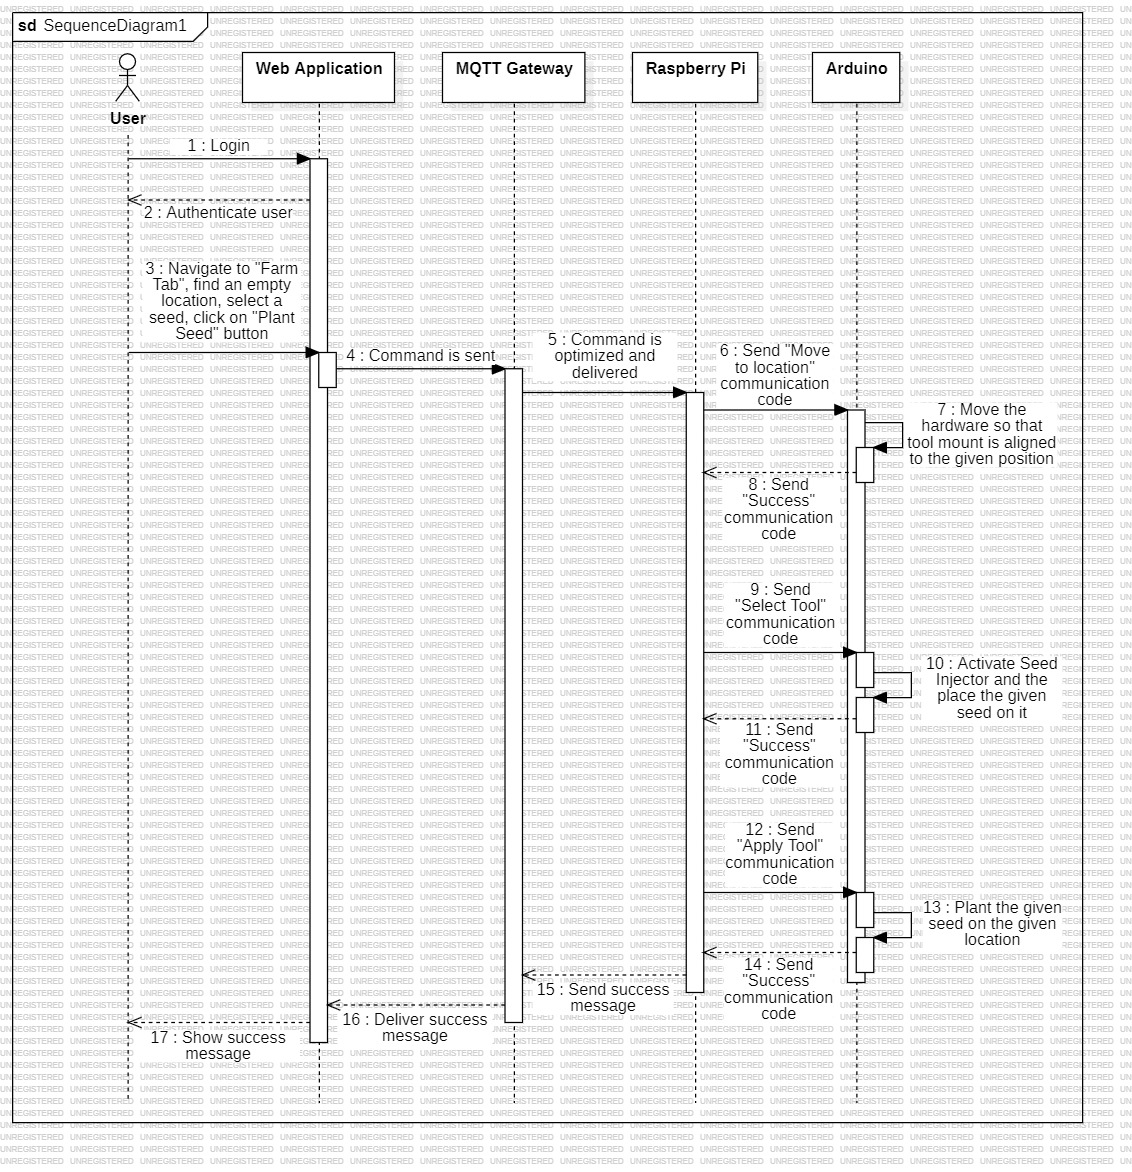
\includegraphics[width=1\linewidth]{Figures/sequence2.jpg}
    \caption{Sequence Diagram for "Plant Seed" Interaction Pattern}
    \label{Sequence2}
\end{figure}
\begin{figure}[htbp]
    \centering
    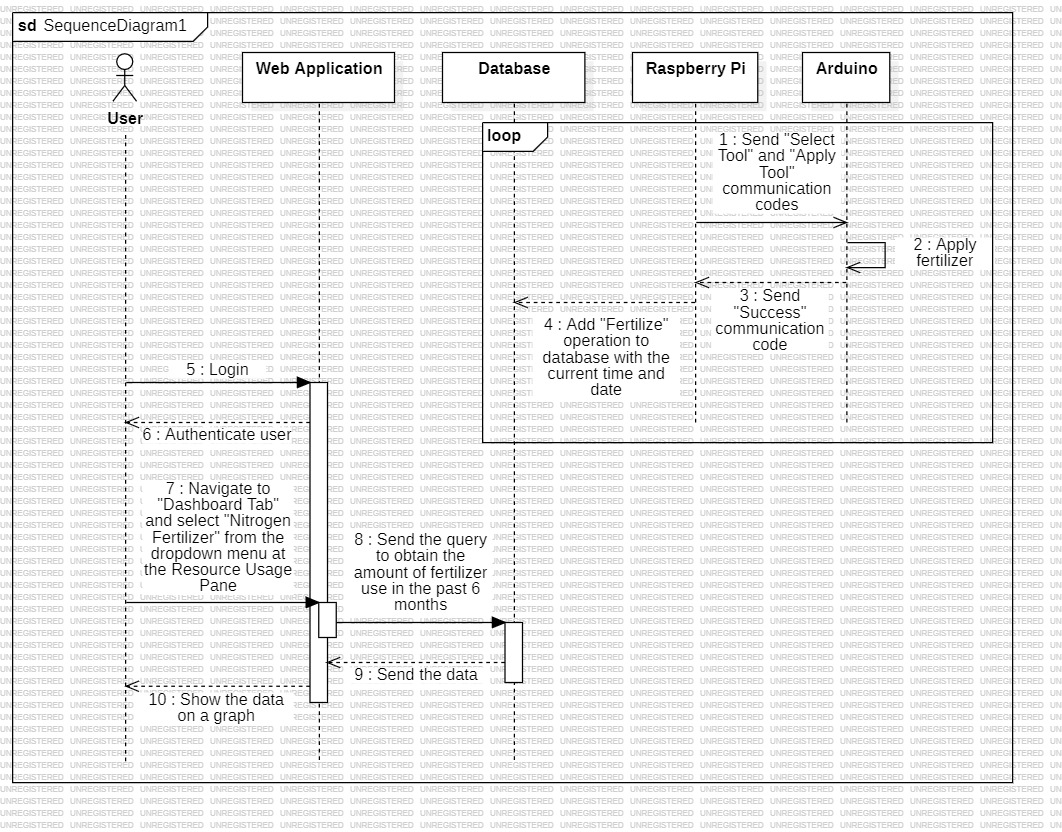
\includegraphics[width=1\linewidth]{Figures/sequence3.jpg}
    \caption{Sequence Diagram for "Display Fertilizer Usage" Interaction Pattern}
    \label{Sequence3}
\end{figure}
\newpage

\section{Information View}

\subsection{Stakeholders’ uses of this view}
The Information View is instrumental for stakeholders in understanding and managing the flow of data within the system. Here is how various stakeholders might use the Information View:
\begin{itemize}
    \item \textbf{Hobbyist Gardeners and Professional Farmers:} They refer to the Information View to know what kind of data is collected about their farming activities, such as soil conditions, weather data, and crop growth, which helps them in making informed decisions for their farming practices.
    \item \textbf{Educators:} Utilize the Information View to teach students about the types of agricultural data managed by FarmBot, which includes data structures related to plant health, environmental conditions, and automated responses of the FarmBot system.
    \item \textbf{Researchers:} Leverage the Information View to understand the specifics of data collected, stored, and analyzed by FarmBot, aiding in research related to sustainable farming practices, crop yield optimization, and ecosystem impacts.
    \item \textbf{Software Developers:} Use the Information View to comprehend the data architecture of FarmBot, informing their software development to enhance functionalities, create new features, and integrate with third-party data services.
    \item \textbf{System Administrators:} Rely on the Information View for database management, ensuring data integrity, security, and efficient data flow from sensors to user interfaces and vice versa. They also use this view to monitor data-related system performance and to troubleshoot issues.
    \item \textbf{Open-Source Contributors and Community Members:} Refer to the Information View to understand the data models and structures that FarmBot uses, which helps them contribute effectively to the project by suggesting improvements or developing new data-driven features.
\end{itemize}
By understanding the Information View, all stakeholders can ensure that data handling within FarmBot aligns with the system's goals of providing an efficient, user-friendly, and educational automated farming experience.

\newpage
\subsection{Database Class Diagram}
\begin{figure}[htbp]
    \centering
    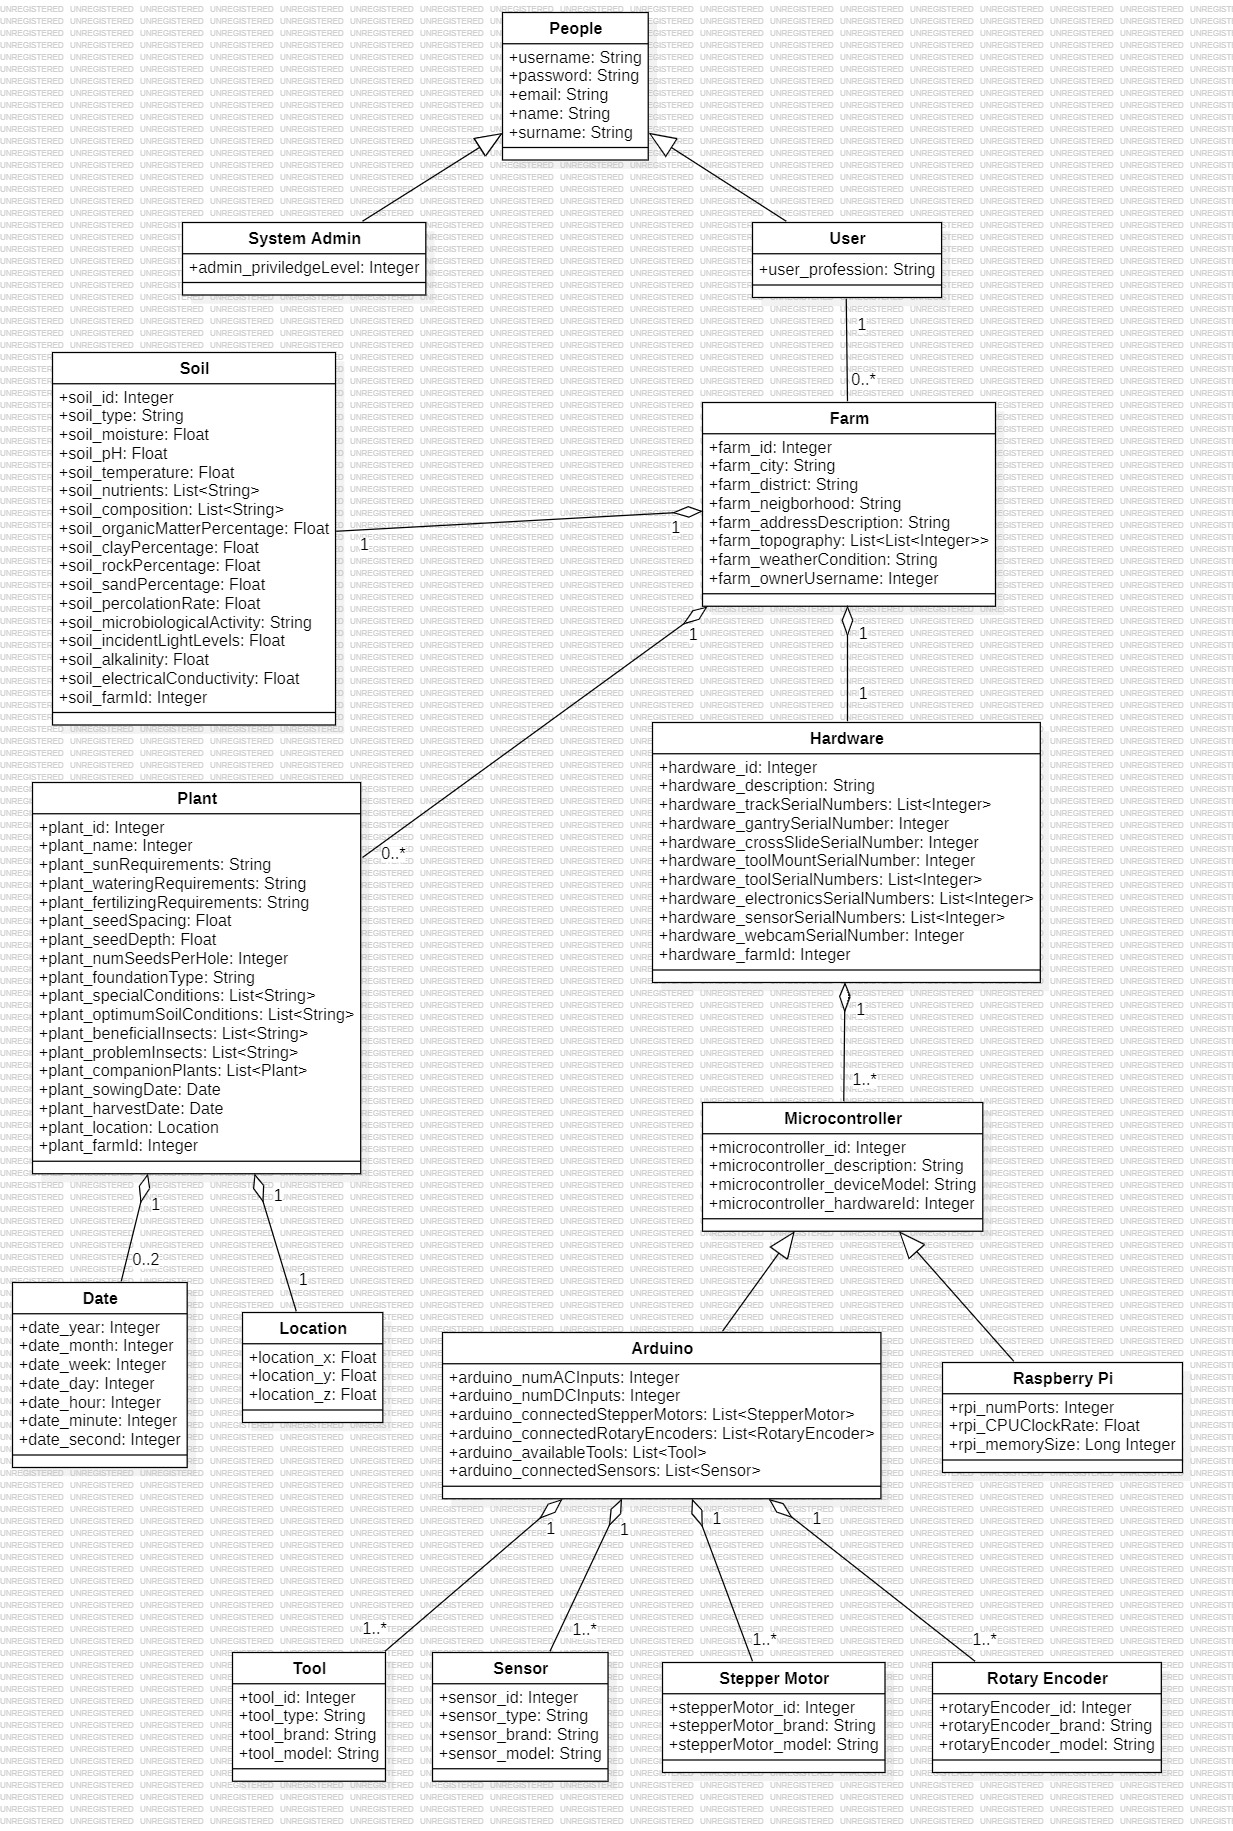
\includegraphics[width=0.7\linewidth]{Figures/database_class_diagram.jpg}
    \caption{Database Class Diagram}
    \label{Database}
\end{figure}
\newpage


\subsection{Operations on Data}
\begin{longtblr}
[
    caption = {CRUD Operations},
    label = {CRUD}
]
{
    colspec = {|X|X|},
    hlines
}
\textbf{Operation} & CRUD Operations  \\ \hline
\textbf{AddUser} & {
    Create: Add a new user to the system.\\
    Read: -\\
    Update: -\\
    Delete: -
}  \\ \hline
\textbf{ChangePriviledgeLevel} & {
    Create: -\\
    Read: -\\
    Update: Change the priviledge level of system administrator.\\
    Delete: -
}  \\ \hline
\textbf{UpdateUserEmail} & {
    Create: -\\
    Read: -\\
    Update: Update a user's email address.\\
    Delete: -
} \\ \hline
\textbf{RemoveUser} & {
    Create: -\\
    Read: -\\
    Update: -\\
    Delete: Delete a user from the system.
}  \\ \hline
\textbf{RegisterSoilData} & {
    Create: Register new soil data into the system.\\
    Read: -\\
    Update: -\\
    Delete: -
} \\ \hline
\textbf{UpdateSoilComposition} & {
    Create: -\\
    Read: -\\
    Update: Arrange the composition of soil by changing organic matter, clay, rock, and sand percentages.\\
    Delete: -
} \\ \hline
\textbf{DeleteSoilData} & {
    Create: -\\
    Read: -\\
    Update: -\\
    Delete: Delete specific soil data from the database.
} \\ \hline
\textbf{CreatePlant} & {
    Create: Add a new plant entry with full details.\\
    Read: -\\
    Update: -\\
    Delete: -
} \\ \hline
\textbf{UpdatePlantRequirements} & {
    Create: -\\
    Read: -\\
    Update: Update a plant's sun, watering, and fertilizer requirements.\\
    Delete: -
} \\ \hline
\textbf{GetSowingDate} & {
    Create: -\\
    Read: Read the sowing date of a plant.\\
    Update: -\\
    Delete: -
} \\ \hline
\textbf{GetHarvestDate} & {
    Create: -\\
    Read: Read the harvest date of a plant.\\
    Update: -\\
    Delete: -
} \\ \hline
\textbf{DeletePlant} & {
    Create: -\\
    Read: -\\
    Update: -\\
    Delete: Remove a plant entry from the database.
} \\ \hline
\textbf{CreateFarm} & {
    Create: Create a farm instance with given data.\\
    Read: -\\
    Update: -\\
    Delete: -
} \\ \hline
\textbf{UpdateFarmAddress} & {
    Create: -\\
    Read: -\\
    Update: Update the address of a farm by changing city, district, neighborhood, etc.\\
    Delete: -
} \\ \hline
\textbf{DeleteFarm} & {
    Create: -\\
    Read: -\\
    Update: -\\
    Delete: Delete a farm instance from the database.
} \\ \hline
\textbf{AddHardware} & {
    Create: Register new hardware in the system.\\
    Read: -\\
    Update: -\\
    Delete: -
} \\ \hline
\textbf{GetSerialNumber} & {
    Create: -\\
    Read: Read the serial number of a hardware part.\\
    Update: -\\
    Delete: -
} \\ \hline
\textbf{RemoveHardware} & {
    Create: -\\
    Read: -\\
    Update: -\\
    Delete: Delete hardware from the system.
} \\ \hline
\textbf{AddMicrocontroller} & {
    Create: Add a new microcontroller configuration.\\
    Read: -\\
    Update: -\\
    Delete: -
} \\ \hline
\textbf{UpdateMicrocontrollerDescription} & {
    Create: -\\
    Read: -\\
    Update: Update the description of an existing microcontroller.\\
    Delete: -
} \\ \hline
\textbf{DeleteMicrocontroller} & {
    Create: -\\
    Read: -\\
    Update: -\\
    Delete: Remove a microcontroller configuration from the system.
} \\ \hline
\textbf{RegisterTool} & {
    Create: Add a new tool to the system.\\
    Read: -\\
    Update: -\\
    Delete: -
} \\ \hline
\textbf{GetToolBrand} & {
    Create: -\\
    Read: Read the brand of a tool.\\
    Update: -\\
    Delete: -
} \\ \hline
\textbf{RemoveTool} & {
    Create: -\\
    Read: -\\
    Update: -\\
    Delete: Delete a tool from the system.
} \\ \hline
\textbf{AddSensor} & {
    Create: Add a new sensor to the database.\\
    Read: -\\
    Update: -\\
    Delete: -
} \\ \hline
\textbf{GetSensorModel} & {
    Create: -\\
    Read: Read the model of a sensor.\\
    Update: -\\
    Delete: -
} \\ \hline
\textbf{DeleteSensor} & {
    Create: -\\
    Read: -\\
    Update: -\\
    Delete: Remove sensor data from the database.
} \\ \hline
\textbf{AddStepperMotor} & {
    Create: Add a new stepper motor to the database.\\
    Read: -\\
    Update: -\\
    Delete: -
} \\ \hline
\textbf{RemoveStepperMotor} & {
    Create: -\\
    Read: -\\
    Update: -\\
    Delete: Remove a stepper motor from the database.
} \\ \hline
\textbf{RegisterRotaryEncoder} & {
    Create: Register a new rotary encoder to the database.\\
    Read: -\\
    Update: -\\
    Delete: -
} \\ \hline
\textbf{DeleteRotaryEncoder} & {
    Create: -\\
    Read: -\\
    Update: -\\
    Delete: Delete a rotary encoder from the database.
}
\end{longtblr}


\section{Deployment View}

\subsection{Stakeholders’ uses of this view}
The Deployment View helps different stakeholders understand how software components are distributed across the hardware and network infrastructure:
\begin{itemize}
    \item \textbf{Hobbyist Gardeners and Professional Farmers:} While they may not interact directly with the Deployment View, understanding that the software runs on both a cloud platform and local devices assures them of the system's resilience and continuous operation, even if their own internet connection is unstable.
    \item \textbf{Educators:} They can use the Deployment View to show students how the FarmBot software is distributed and interacts with various hardware components, from the cloud servers to the Raspberry Pi and Arduino controllers on the physical FarmBot units.
    \item \textbf{Researchers:} Interested in how the deployment of the system can affect data collection and the responsiveness of FarmBot to changes in the environment or in its operational commands.
    \item \textbf{Software Developers:} Utilize the Deployment View to ensure their code is optimized for the environments it will run in, whether it's on the lightweight Raspberry Pi or a robust cloud server, and understand the communication between these nodes.
    \item \textbf{System Administrators:} Rely heavily on the Deployment View to manage the physical and virtual resources that the FarmBot system depends on, ensuring that all components are properly maintained and configured for efficient operation.
    \item \textbf{Open-Source Contributors and Community Members:} May refer to the Deployment View to better understand how their contributions fit into the broader system, ensuring compatibility with the existing infrastructure and identifying areas where improvements can be made.
\end{itemize}
This view is essential for ensuring that the FarmBot system's deployment is aligned with its performance requirements and can scale to meet growing demand while remaining robust and reliable.

\newpage
\subsection{Deployment Diagram}
\begin{figure}[htbp]
    \centering
    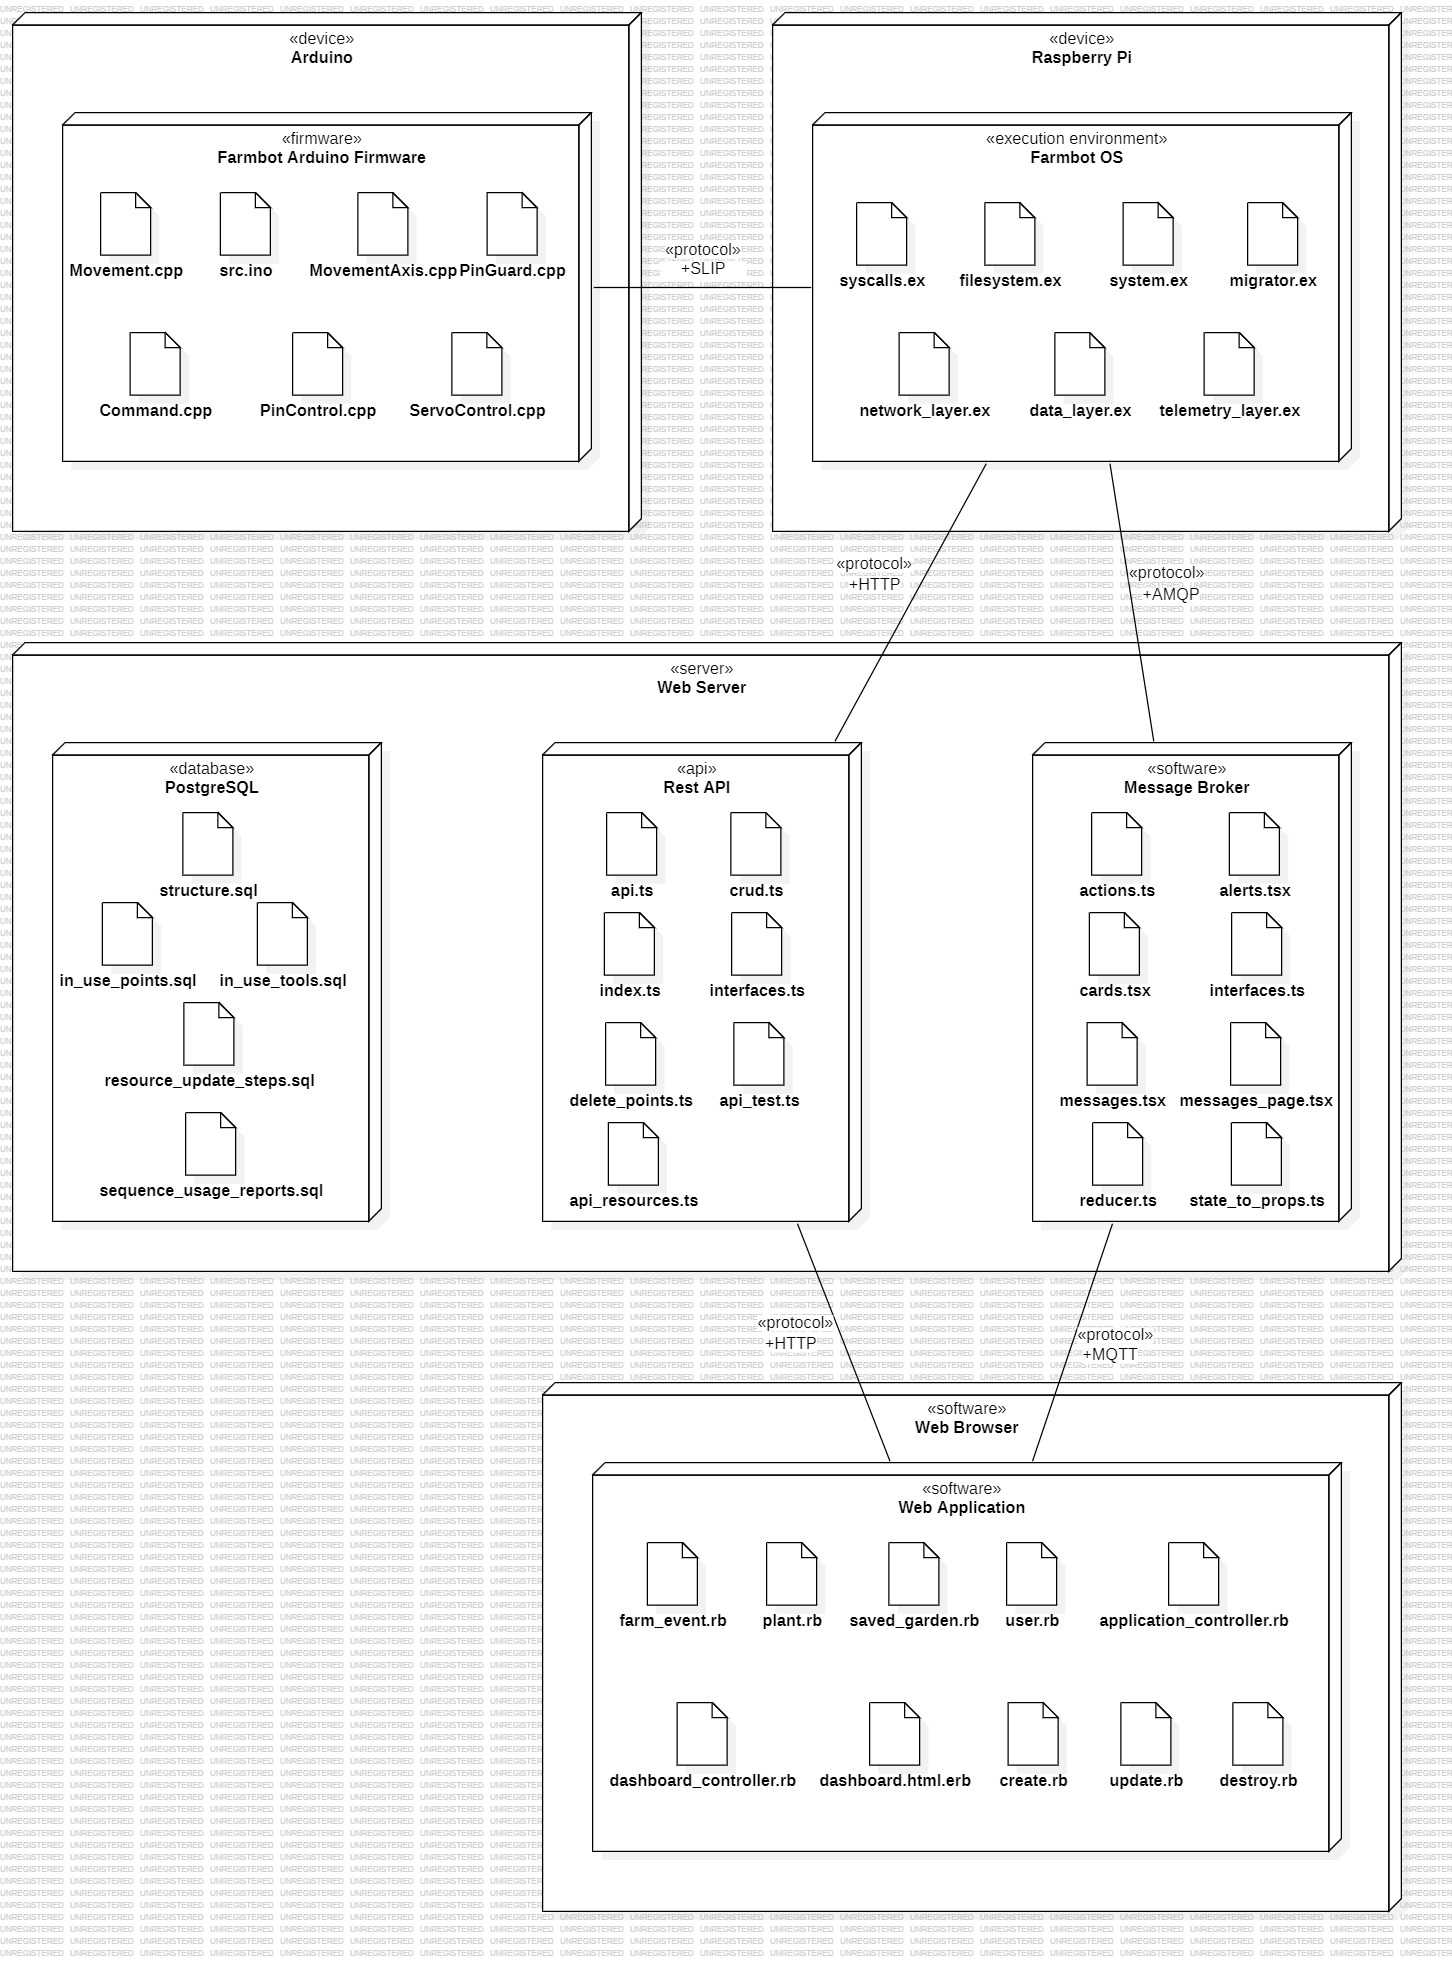
\includegraphics[width=0.7\linewidth]{Figures/deployment_diagram.jpg}
    \caption{Deployment Diagram}
    \label{Deployment}
\end{figure}
\newpage
The deployment diagram for FarmBot showcases the system’s infrastructure and interconnections, depicting the distribution of software components across various hardware devices and the specific protocols used for communication. The diagram is organized into several key areas, each highlighting different aspects of the FarmBot system.
\begin{itemize}
    \item \textbf{Arduino:} Hosts the FarmBot Arduino Firmware, executing various C++ files such as Movement.cpp, Command.cpp, PinControl.cpp, and ServoControl.cpp that manage movement axes, command interpretation, pin control, and servo management, crucial for the physical operations of FarmBot.
    \item \textbf{Raspberry Pi:} Runs FarmBot OS, which includes critical modules like syscall.ex, filesystem.ex, system.ex, and migrator.ex, alongside network\_layer.ex, data\_layer.ex, and telemetry\_layer.ex. These modules handle system calls, file management, data processing, and network communication using HTTP and AMQP protocols to interact with other system components.
    \item \textbf{Web Server:} Divided into three main segments:
        \begin{itemize}
            \item \textbf{Database:} Utilizes PostgreSQL for data storage, handling files like structure.sql and various SQL scripts for updating and managing resources and sequences.
            \item \textbf{REST API:} Supports operations defined in files like crud.ts, index.ts, and api.ts, which facilitate data handling and interaction with the web application.
            \item \textbf{Message Broker:} This component functions as the middleware facilitating asynchronous communication across the system. It manages actions, alerts, and message parsing as defined in files like actions.ts, alerts.tsx, and messages.tsx, crucial for efficient state management and event handling across FarmBot’s distributed environment.
        \end{itemize}
    \item \textbf{Web Browser:} Represents the client-side of the FarmBot system, hosting the Web Application with Ruby on Rails files like farm\_event.rb, plant.rb, user.rb, which are crucial for rendering the user interface and handling user interactions, data display, and direct management of farming events.
\end{itemize}
Communication across these components is maintained through various protocols:
\begin{itemize}
    \item HTTP/HTTPS for secure web interactions,
    \item AMQP for robust messaging between the Raspberry Pi and the web server,
    \item MQTT for lightweight messaging particularly useful for IoT devices like FarmBot.
\end{itemize}
This deployment diagram effectively outlines the operational blueprint of FarmBot, illustrating how various software and hardware components integrate and communicate to create a functional autonomous farming system. This structure ensures that FarmBot can efficiently execute agricultural tasks while providing users with real-time control and monitoring capabilities.

\newpage
\section{Design Rationale}
\textbf{Design Rationale for Context View}\\
For the Context View of FarmBot, the decision was made to integrate the system with the OpenFarm.cc API and other external interfaces like GitHub. The rationale was to ensure that FarmBot benefits from a vast, shared knowledge base for plant data and collaborative improvement of its software, which aligns with the open-source nature of the project. Leveraging GitHub fosters an active development community and continuous enhancement of the platform, essential for adapting to the evolving needs of users and technology.\\\\
\textbf{Design Rationale for Functional View}\\
The Functional View of FarmBot divides the system into distinct components, such as the User Interface, System Admin Interface, and interactions with external entities like OpenFarm.cc and GitHub. This separation allows clear representation of responsibilities, improving system coherence and easing both development and future enhancements. Focusing on modular design also supports ease of maintenance and scalability, essential for the diverse applications of FarmBot users, ranging from hobbyists to research institutions.\\\\
\textbf{Design Rationale for Information View}\\
The Information View was designed to organize and manage data related to farming operations in a structured, relational model. This approach facilitates the efficient handling of complex and interrelated agricultural data. By structuring data hierarchically, FarmBot ensures quick access and robust data integrity, making the system reliable and trustworthy for users who rely on it for precision farming.\\\\
\textbf{Design Rationale for Deployment View}\\
In the Deployment View, the decision to deploy key components of the FarmBot system on scalable servers was driven by the need for high availability and robustness. Such a deployment ensures that FarmBot's services are reliable and continuously available to users worldwide. Moreover, the use of servers enables FarmBot to handle varying loads dynamically, which is critical during peak farming seasons or when integrating with third-party services for extended functionality.